\documentclass[10pt,twocolumn,a4paper]{article}
\usepackage[utf8]{inputenc}
\usepackage[spanish,es-tabla]{babel}
\usepackage[left=1.5cm,right=1.5cm,top=1.45cm,bottom=1.45cm,columnsep=0.55cm]{geometry}
\usepackage{amsmath,amssymb}
\usepackage{graphicx}
\usepackage{booktabs}
\usepackage{titlesec}
\usepackage{array}
\usepackage{xcolor}

\titleformat{\section}[block]{\normalsize\bfseries\filcenter}{\Roman{section}.}{0.4em}{}
\titlespacing*{\section}{0pt}{3.0pt plus 1pt minus 1pt}{1.5pt plus 1pt minus 1pt}

\setlength{\abovedisplayskip}{3pt plus 1pt minus 1pt}
\setlength{\belowdisplayskip}{3pt plus 1pt minus 1pt}
\setlength{\textfloatsep}{5pt plus 1pt minus 1pt}
\setlength{\floatsep}{4pt plus 1pt minus 1pt}
\setlength{\intextsep}{4pt plus 1pt minus 1pt}

\newsavebox{\logobox}

\begin{document}

\sbox{\logobox}{
\includegraphics[width=1.55cm]{Assets/logounillanos.png}}

\twocolumn[{%
  \begin{tabular*}{\textwidth}{@{\extracolsep{\fill}}m{1.6cm}m{13.2cm}m{1.5cm}}
    \centering\usebox{\logobox} &
    \centering
    {\fontsize{10.5pt}{12pt}\selectfont\textbf{UNIVERSIDAD DE LOS LLANOS}}\\[0.05cm]
    {\fontsize{8.8pt}{10.5pt}\selectfont Facultad de Ciencias Básicas e Ingeniería --- Ingeniería en Sistemas}\\[0.03cm]
    {\fontsize{8.2pt}{9.8pt}\selectfont\textit{Estructuras de Datos (Corte 3: Grafos y Optimización) --- Villavicencio, Colombia}} &
    \rule{1.5cm}{0pt}
  \end{tabular*}
  
  \vspace{0.20cm}
  \centering
  {\fontsize{11.5pt}{13.5pt}\selectfont\textbf{MODELADO MEDIANTE GRAFOS MULTIMODALES Y OPTIMIZACIÓN DE LA CADENA DE FRÍO PARA PESCA ARTESANAL EN PUERTO GAITÁN, META}}\\[0.15cm]
  {\fontsize{8.8pt}{10.5pt}\selectfont\textbf{Yair Armando Ospino Herrera} (160005565) \quad $\bullet$ \quad \textbf{Harold Esteban Padilla Díaz} (160005567)}\\[0.05cm]
  {\fontsize{8.2pt}{9.8pt}\selectfont\textit{Facultad de Ciencias Básicas e Ingeniería --- Ingeniería en Sistemas, Universidad de los Llanos, Villavicencio, Colombia}}\\[0.18cm]
  
  \noindent\fcolorbox{black!15}{black!3}{%
    \parbox{0.98\textwidth}{%
      \centering\textbf{\small Resumen}\\[0.06cm]
      \fontsize{8.2pt}{9.8pt}\selectfont
      En este trabajo se modela la red logística y comercial pesquera artesanal de Puerto Gaitán (Meta) como un grafo dirigido ponderado multimodal ($|V| = 25$ vértices y $|E| = 41$ aristas) con el propósito de erradicar la pérdida poscaptura de cachama de río (\textit{Colossoma macropomum}), la cual alcanza el $40\%$ debido a temperaturas de $30\,^\circ\text{C}$ y a la carencia de refrigeración continua. A partir del censo de 33 fichas cartográficas de 7 asociaciones pesqueras ($265.8\text{ kg/día}$), la red hidrográfica real del IGAC ($12,413$ nodos en \textit{rios.shp}) y ruteo vial OSRM sobre la Ruta Nacional 40, se codificaron desde cero en Python 3.14 los algoritmos de Dijkstra (con heap binario), Bellman-Ford, Floyd-Warshall, BFS, DFS y el Problema de Localización de Instalaciones (FLP Greedy). Se dio solución rigurosa a las cuatro incógnitas operacionales: (i) BFS determinó que el $85.7\%$ de los puertos pesqueros accede a un nodo de acopio o frío en 1 o 2 saltos topológicos; (ii) Dijkstra y DFS fijaron itinerarios óptimos hacia Bogotá D.C. ($\sim 295\text{ km}$) limitando la exposición sin frío a un intervalo de $0.08\text{ a }2.20\text{ h}$, cumpliendo ampliamente el umbral sanitario de $4.0\text{ h}$ de la FAO; (iii) FLP demostró que la apertura del Centro Frío Puerto Gaitán ($F02$, $\$3.0\text{M COP/mes}$) garantiza el $100\%$ de cobertura regional a un costo unitario de $\$59,080\text{ COP/kg}$, ahorrando $\$10.0\text{M COP}$ mensuales respecto a la operación de tres plantas; y (iv) el análisis de regresión lineal empírica estableció una tasa fluvial de $3.64\text{ min/km}$ ($v = 16.5\text{ km/h}$, $R^2 = 0.999$) frente a $0.92\text{ min/km}$ terrestre, demostrando que la navegación fluvial representa el cuello de botella físico de la cadena.\\[0.06cm]
      \textbf{Palabras clave---}Cadena de frío, caminos mínimos, \textit{Colossoma macropomum}, Dijkstra, grafos dirigidos, localización de instalaciones, multimodalidad, OSRM.
    }%
  }
  \vspace{0.25cm}
}]

\section{Introducción}
La pesca artesanal en el municipio de Puerto Gaitán (Meta) constituye la base económica de comunidades ribereñas en los ríos Meta, Manacacías e Iteviare. La captura se concentra en especies reofílicas de alto valor comercial, predominantemente la cachama de río (\textit{Colossoma macropomum}). No obstante, las temperaturas ambiente medias de la Orinoquía ($30\,^\circ\text{C}$) aceleran el rigor mortis y la proliferación microbiana en el tejido muscular, provocando pérdidas poscaptura de hasta el $40\%$ antes de alcanzar los mercados urbanos [1, 2].

Desde la perspectiva formal de las estructuras de datos, un sistema multimodal de transporte se modela rigurosamente como un grafo dirigido ponderado $G = (V, E)$, representado en memoria mediante listas de adyacencia sobre tablas hash con costo espacial óptimo $\mathcal{O}(|V| + |E|)$ [3]. Para capturar con fidelidad la física del transporte, cada arista dirigida $e = (u, v) \in E$ se pondera mediante una función multicriterio normalizada de seis componentes:
\begin{equation}
    w(e) = 0.25\,t + 0.20\,c + 0.20\,r + 0.10\,p + 0.10\,(1-\text{conf}) + 0.05\,\text{ret}
\end{equation}
donde $t$ es el tiempo de tránsito normalizado, $c$ el costo de flete, $r$ la confiabilidad de la vía, $p$ la penalización por deterioro y $\text{ret}$ las demoras fijas en muelles. La degradación microbiológica acumulada $D_{\text{acum}}$ a $30\,^\circ\text{C}$ sigue una cinética lineal en función del tiempo de exposición al ambiente [2]:
\begin{equation}
    D_{\text{acum}} = D_0 + \sum_{i=1}^n k_i \cdot t_i
\end{equation}
donde la constante de descomposición base es $k = 2.5\%\text{/h}$ y asciende a $k_D = 1.5\,k = 3.75\%\text{/h}$ en tramos destapados sin sombra (zonas críticas $D$). El límite máximo de inocuidad alimentaria fijado por la FAO para pescado tropical fresco sin refrigerar es $t_{\max} = 4.0\text{ h}$ ($240\text{ min}$) [1]. Al arribar a un centro de frío ($F$), el producto desciende a $0\,^\circ\text{C}$ (relación hielo/pescado 1:1), reiniciando el reloj térmico a $0.0\text{ h}$ y asegurando una vida útil comercial de hasta $360\text{ h}$ (15 días) [1].

\textbf{Estado del arte:} El análisis de redes y caminos mínimos se originó con los aportes seminales de Dijkstra (1959), Bellman-Ford (1958) y Floyd-Warshall (1962), orientados a distancias escalares sobre topologías discretas [3]. Posteriormente, Hakimi (1964) y Laporte et al. (2019) formalizaron el Problema de Localización de Instalaciones (FLP / $p$-mediana) para determinar la apertura óptima de infraestructuras minimizando inversión fija y acarreo [4, 5]. En años recientes, la optimización de cadenas agroalimentarias ha migrado hacia la articulación de grafos computacionales con Sistemas de Información Geográfica (SIG), integrando hidrografía vectorial con motores de ruteo vial como OSRM para suprimir las distorsiones de la distancia euclidiana [5].

\textbf{Restricciones del modelo:} El corredor logístico analizado presenta cuatro restricciones fundamentales: (i) la navegación fluvial en canoa artesanal ($v_{\text{canoa}} \approx 16.5\text{ km/h}$) exhibe una incertidumbre propagada de $\Delta t = \pm 0.15 \cdot t$ por corrientes estacionales y palizadas; (ii) los muelles de transbordo ($M$) imponen una demora obligatoria de $+0.25\text{ h}$ a la intemperie; (iii) los hábitats protegidos ($H$) poseen estatus de conservación ambiental estricto, vetados como nodos de tránsito; y (iv) la red eléctrica trifásica indispensable para compresores frigoríficos solo existe en nodos urbanos seleccionados ($F01, F02, F03$).

El presente artículo resuelve cuatro incógnitas operacionales: (i) calcular con BFS el centro de acopio o frío más próximo en saltos mínimos desde cada puerto; (ii) trazar mediante Dijkstra y DFS los itinerarios óptimos hacia Bogotá D.C. cuantificando la degradación térmica; (iii) optimizar con FLP Greedy la apertura de plantas frigoríficas minimizando la inversión total; y (iv) deducir experimentalmente las ecuaciones cinemáticas de transporte mediante regresión lineal $t(d)$.

\section{Sección Experimental y Metodología}
El desarrollo del proyecto se ejecutó en Python 3.14 con una arquitectura orientada a objetos modular, implementando las estructuras de datos y algoritmos desde cero, sin utilizar librerías de cálculo en grafos. El procedimiento experimental comprendió tres fases continuas:

\textbf{1. Adquisición cartográfica y catálogo de red:} Con base en el censo de 33 fichas de campo levantadas con pescadores artesanales en Puerto Gaitán y Puerto López, se caracterizaron 7 asociaciones pesqueras (captura neta: $265.75\text{ kg/día}$). Se estructuraron 25 vértices clasificados en 7 tipos funcionales ($P$: 7 puertos de captura, $M$: 3 muelles de transbordo, $A$: 3 acopios rurales, $F$: 3 nodos frigoríficos candidatos, $D$: 2 zonas críticas de deterioro térmico, $H$: 2 hábitats de reserva ecológica y $V$: 5 mercados mayoristas con coordenadas verificadas en Puerto Gaitán, Villavicencio y Bogotá) interconectados por 41 aristas dirigidas.

\textbf{2. Construcción del doble grafo y ruteo geográfico:} Se implementó el Grafo Logístico Principal ($|V|=25, |E|=41$) mediante listas de adyacencia sobre tablas hash con complejidad temporal $\mathcal{O}(1)$ en búsquedas de vecindad. En paralelo, se procesó el shapefile hidrográfico oficial del IGAC (\textit{rios.shp}), construyendo un Grafo Fluvial Topológico continuo con $12,413$ nodos cuantizados a 5 decimales (precisión submétrica) y $24,790$ aristas de cauce, indexadas mediante una cuadrícula espacial hash de 447 celdas ($0.05^\circ \times 0.05^\circ$) para resolver con exactitud la navegación por meandros. Las aristas terrestres sobre la Ruta Nacional 40 se computaron con la API del motor OSRM, almacenando 41 polilíneas en caché JSON local.

\begin{figure}[htbp]
    \centering
    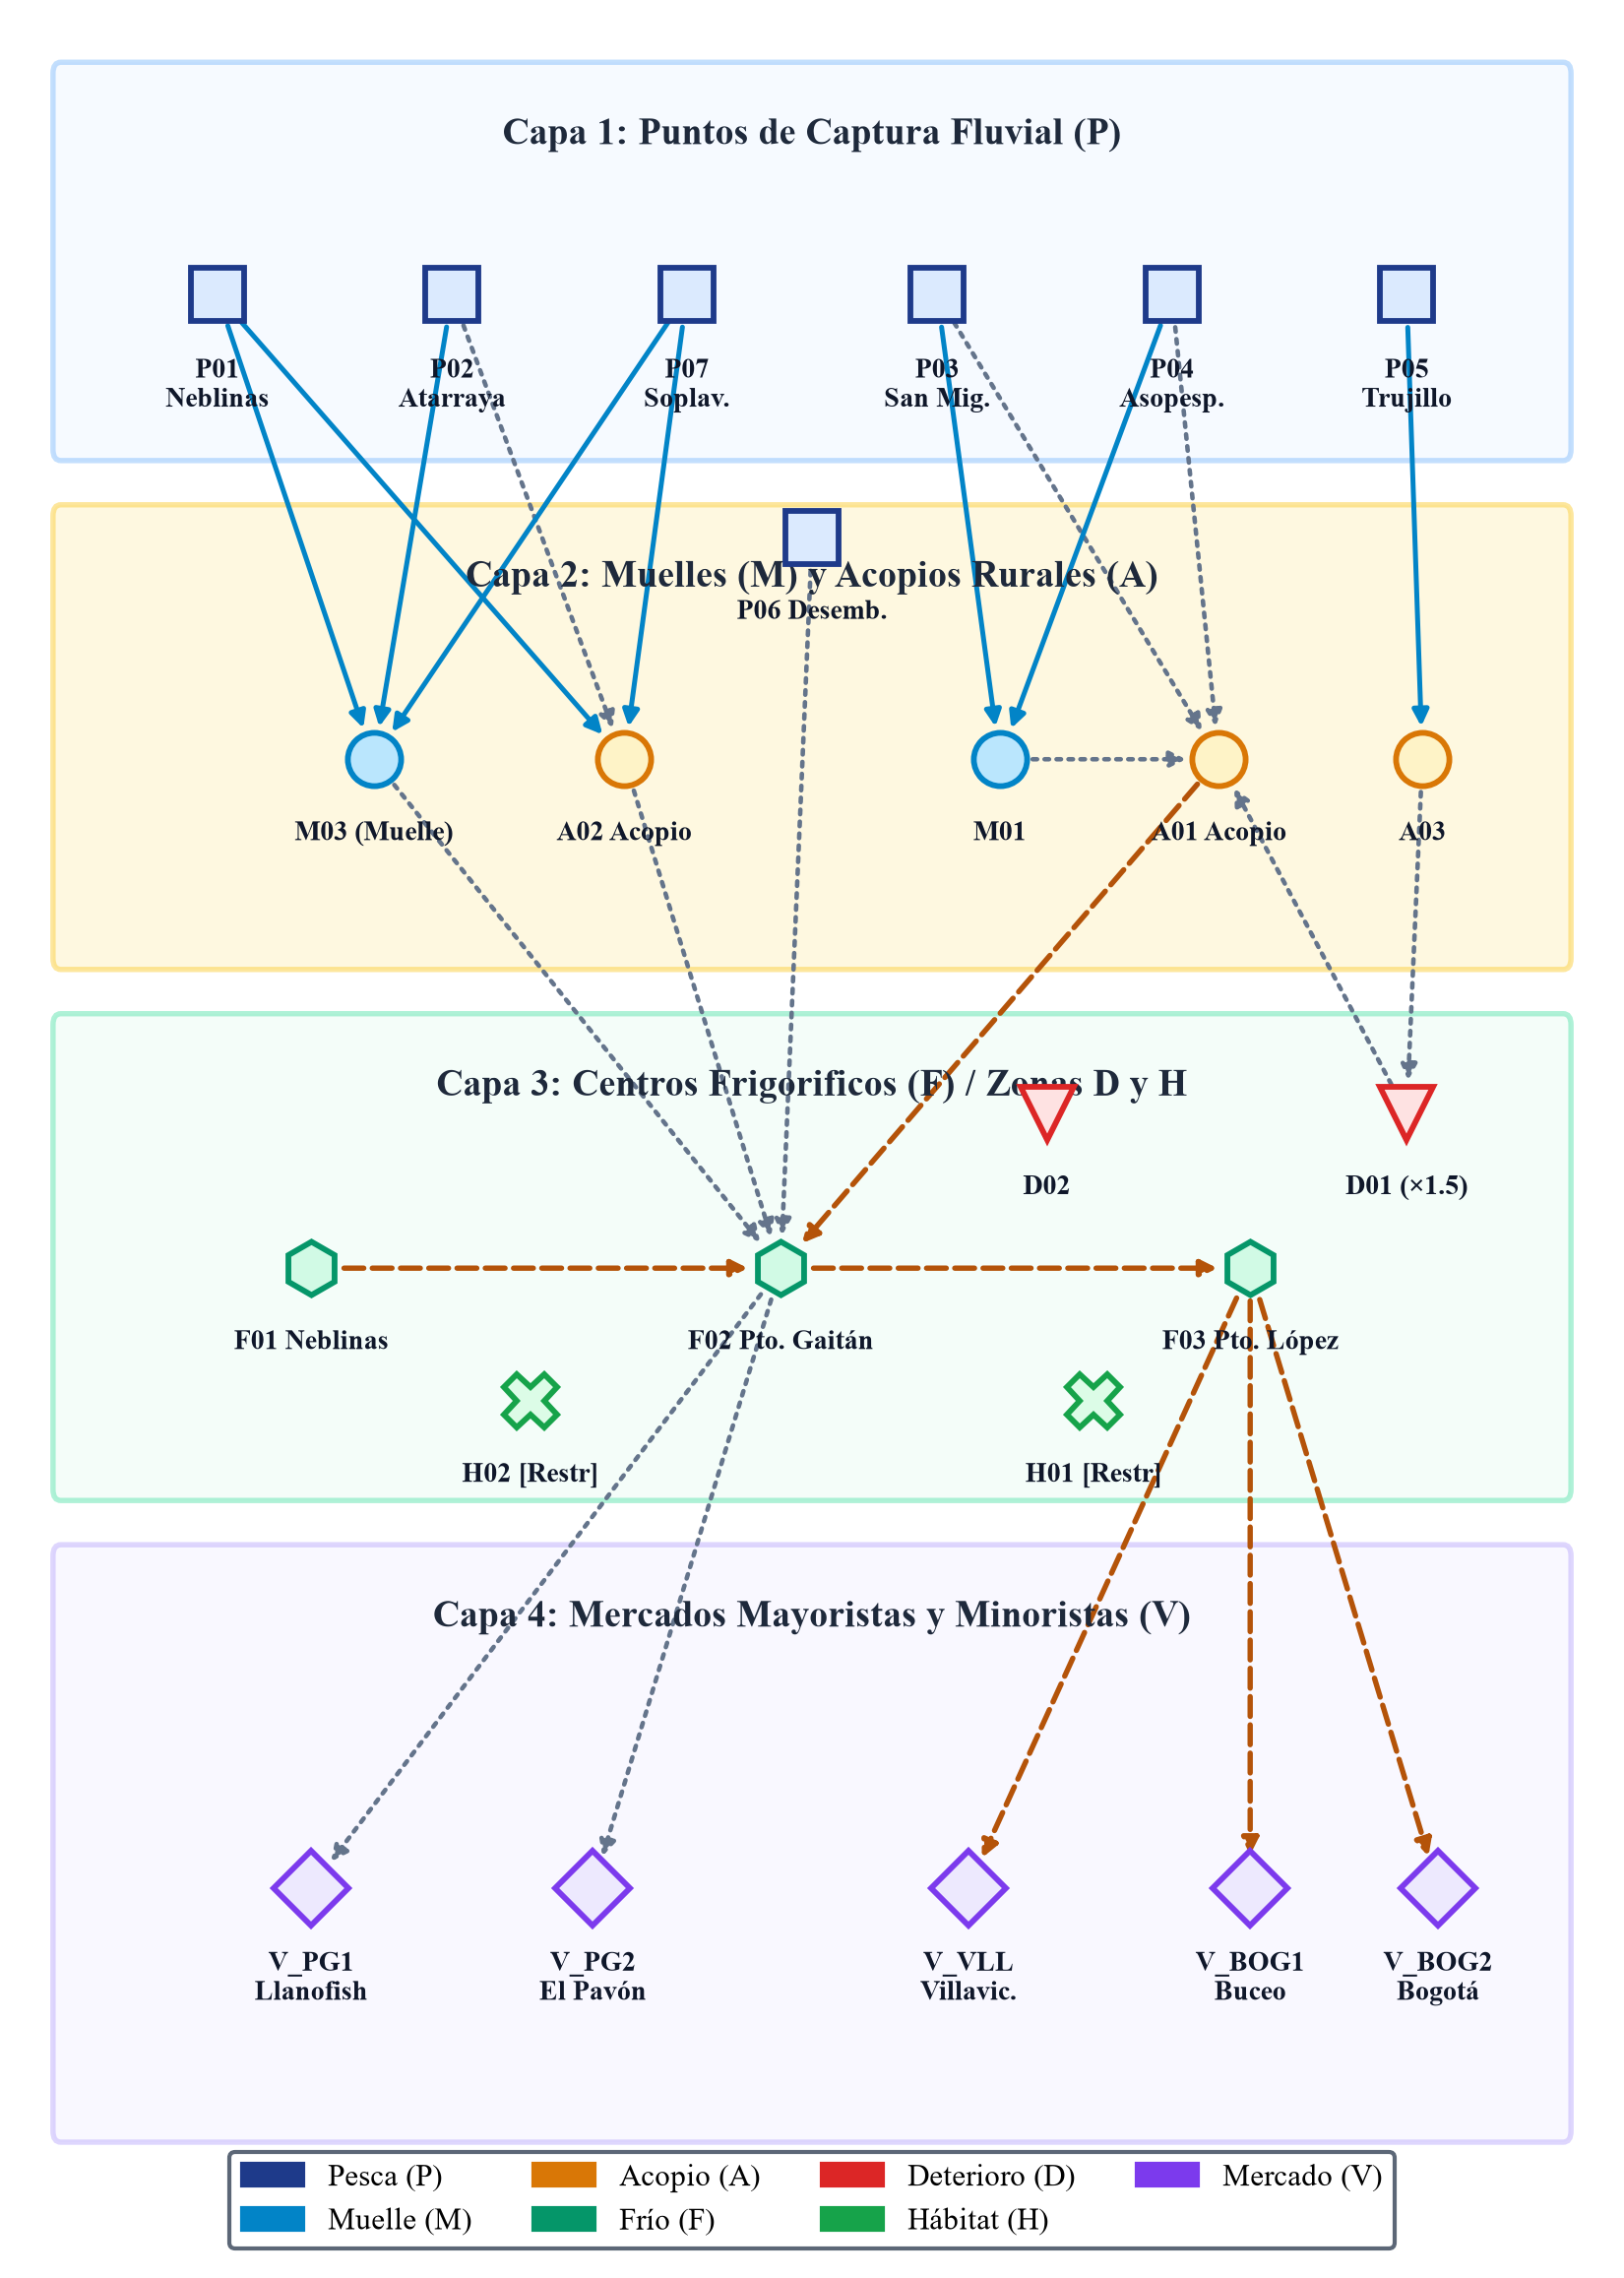
\includegraphics[width=0.68\linewidth]{Assets/figura_1_topologia_col.png}
    \caption{Topología del grafo logístico multimodal (25 vértices y 41 aristas) en 4 capas funcionales con restricciones ambientales $H$ y térmicas $D$.}
    \label{fig:topologia}
\end{figure}

\textbf{3. Ejecución algorítmica y control de calidad:} Se codificaron manualmente: Dijkstra con cola de prioridad basada en montículo binario (\textit{heapq}), Bellman-Ford con verificación de ciclos negativos, Floyd-Warshall sobre matriz adyacente, BFS con cola FIFO (\textit{deque}), DFS recursivo con retroceso y FLP Greedy con evaluación multicriterio. El entorno de trabajo contó con una suite de 40 pruebas unitarias automatizadas en pytest, visualizador cartográfico Leaflet/Folium y sistema de coordenadas WGS 84.

\section{Resultados y Análisis}
\textbf{Clasificación de variables del sistema:}
(i) \textit{Variables directas:} coordenadas geográficas WGS 84 (latitud, longitud), masa de captura pesquera diaria $m_P$ [$\text{kg/día}$], costos fijos de apertura frigorífica [$\text{COP/mes}$], distancias métricas de cauce y carretera $d_i$ [$\text{km}$] y tiempos base de viaje $t_i$ [$\text{h}$];
(ii) \textit{Variables indirectas:} saltos topológicos de transbordo (BFS), ponderaciones multicriterio de arista $w(e)$, tiempo acumulado sin refrigeración $t_{\text{sinFrío}}$, incertidumbre temporal propagada $\Delta t$, degradación biológica del pescado $D_{\text{acum}}$ [$\%$], costo unitario total [$\text{COP/kg}$] y coeficientes del ajuste por mínimos cuadrados.

La propagación de incertidumbre en el transporte fluvial $\Delta t$ provocada por variaciones de corriente y estiaje se calculó formalmente mediante la relación de error relativo [6]:
\begin{equation}
    \Delta t = t \cdot \frac{\Delta v_{\text{canoa}}}{v_{\text{canoa}}} = 0.15 \cdot t
\end{equation}

\textbf{Resolución de las Incógnitas 1 y 2 (BFS, Dijkstra y DFS):} La Tabla~\ref{tab:ruteo} sintetiza los resultados cuantitativos de la Incógnita 1 (acopio o frío más cercano en saltos mínimos mediante BFS) y de la Incógnita 2 (itinerario óptimo y deterioro de cachama a Bogotá D.C. mediante Dijkstra y DFS).

\begin{table}[htbp]
\centering
\small
\caption{Resolución Incógnitas 1 y 2: Proximidad BFS, itinerarios Dijkstra a Bogotá y degradación de cachama.}
\label{tab:ruteo}
\resizebox{\columnwidth}{!}{%
\begin{tabular}{|l|c|c|l|c|c|}
\hline
\textbf{Punto} & \textbf{kg/d} & \textbf{BFS} & \textbf{Itinerario a Bogotá} & \textbf{1er Frío} & \textbf{Det.} \\ \hline
$P01$ Neblinas & $65.8$ & 2 ($A02$) & $P01 \to M03 \to F02 \to \text{Bog}$ & $0.48 \pm 0.07\text{ h}$ & $1.20\%$ \\ \hline
$P02$ Atarraya & $40.0$ & 1 ($A02$) & $P02 \to M03 \to F02 \to \text{Bog}$ & $0.43 \pm 0.06\text{ h}$ & $1.08\%$ \\ \hline
$P03$ S. Miguel & $25.0$ & 1 ($A01$) & $P03 \to A01 \to F02 \to \text{Bog}$ & $0.25 \pm 0.04\text{ h}$ & $0.62\%$ \\ \hline
$P04$ Asopespor & $20.0$ & 1 ($A01$) & $P04 \to A01 \to F02 \to \text{Bog}$ & $0.40 \pm 0.06\text{ h}$ & $1.00\%$ \\ \hline
$P05$ Trujillo & $30.0$ & 1 ($A03$) & $P05 \to A03 \to D01 \to \text{Bog}$ & $2.20 \pm 0.33\text{ h}$ & $6.38\%$ \\ \hline
$P06$ Desemb. & $50.0$ & 1 ($F02$) & $P06 \to F02 \to F03 \to \text{Bog}$ & $0.08 \pm 0.01\text{ h}$ & $0.20\%$ \\ \hline
$P07$ Soplav. & $35.0$ & 2 ($A02$) & $P07 \to M03 \to F02 \to \text{Bog}$ & $0.38 \pm 0.06\text{ h}$ & $0.95\%$ \\ \hline
\end{tabular}%
}
\end{table}

\begin{figure}[htbp]
    \centering
    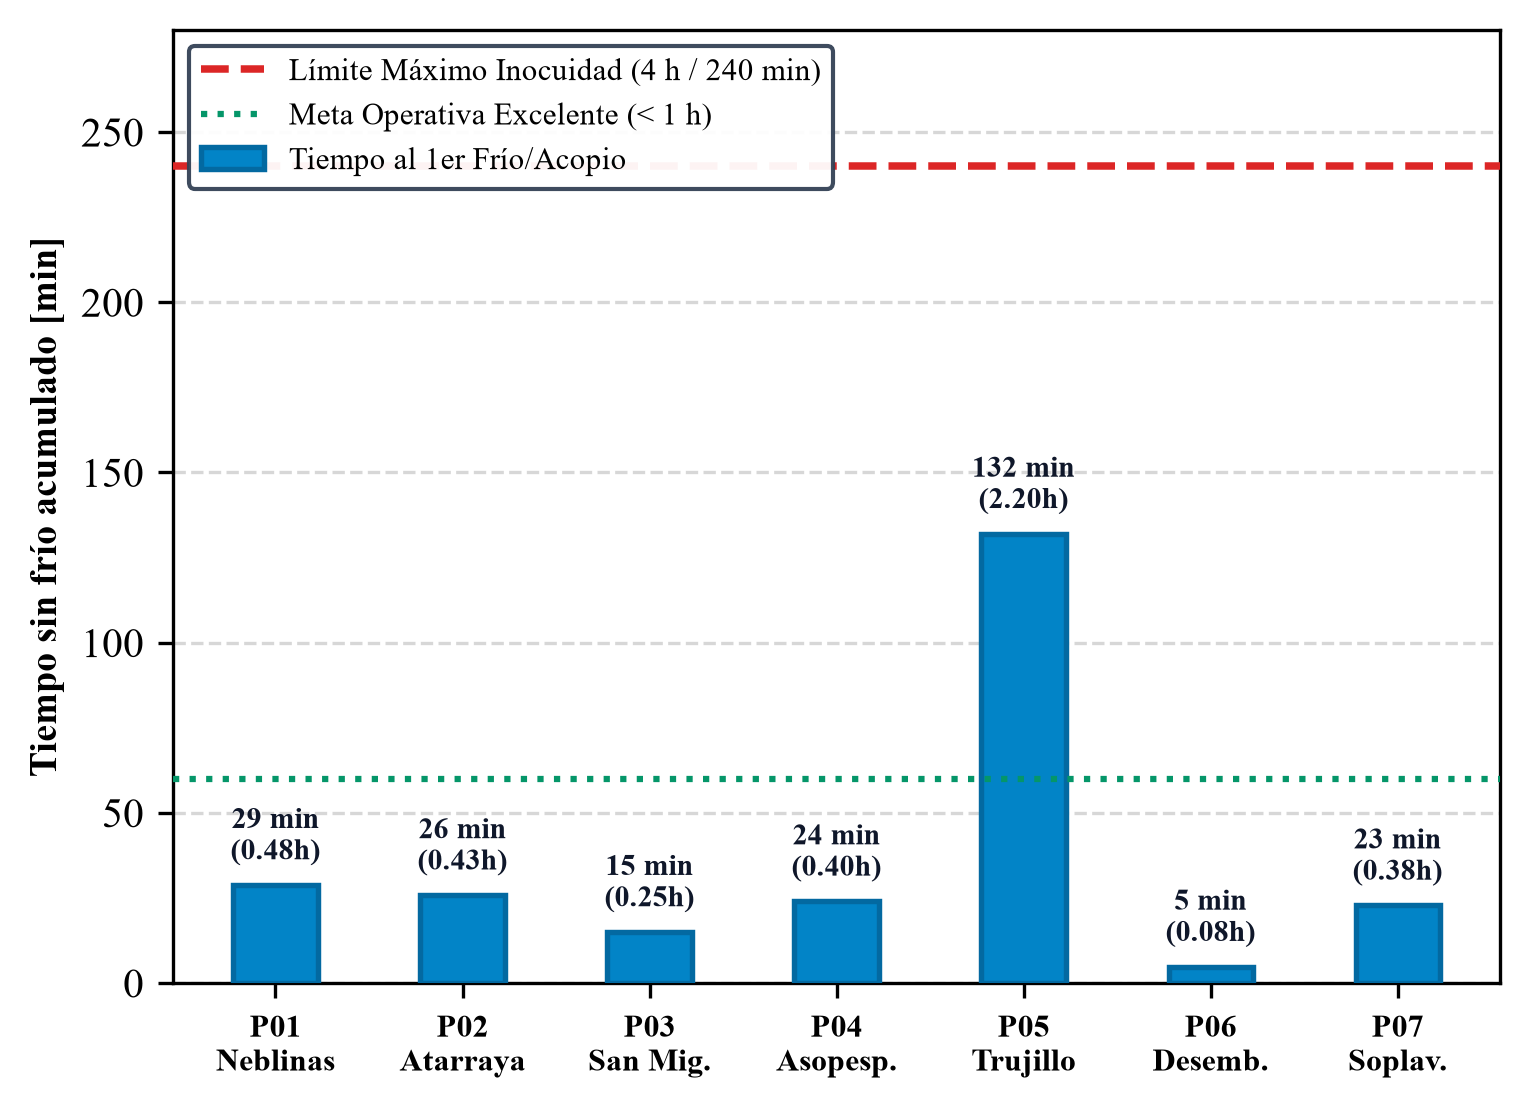
\includegraphics[width=0.68\linewidth]{Assets/grafica_1_bfs_col.png}
    \caption{Tiempo acumulado sin refrigeración por punto de captura frente al umbral crítico sanitario de 4.0 h de la FAO.}
    \label{fig:grafica_bfs}
\end{figure}

El análisis de la Tabla~\ref{tab:ruteo} y la Fig.~\ref{fig:grafica_bfs} demuestra que la totalidad de los puertos alcanza una instalación de frío muy por debajo del umbral crítico de $4.0\text{ h}$. Seis de los siete nodos acceden a refrigeración en menos de $0.50\text{ h}$ ($30\text{ min}$). El caso de mayor aislamiento geográfico corresponde a Puerto Trujillo ($P05$), el cual debe navegar $63\text{ km}$ sobre el río Iteviare y superar la sabana destapada $D01$, acumulando $2.20 \pm 0.33\text{ h}$ sin frío y un deterioro muscular de $6.38\%$, preservando plenamente su aptitud comercial [1]. Adicionalmente, el costo ambiental infinito asignado a los hábitats protegidos desvió eficazmente el tráfico de $P04$, evitando bordear la reserva ecológica $H01$.

\textbf{Resolución de la Incógnita 3 (Localización Óptima FLP):} El algoritmo FLP Greedy evaluó cinco configuraciones operacionales (Tabla~\ref{tab:flp} y Fig.~\ref{fig:grafica_flp}). La solución óptima seleccionó como única sede el Centro Frío Puerto Gaitán ($F02$, $\$3.0\text{M COP/mes}$), el cual asegura el $100\%$ de cobertura regional con un costo unitario consolidado de $\$59,080\text{ COP/kg}$, erradicando el sobrecosto de $\$10.0\text{M COP}$ mensuales derivado de operar tres plantas simultáneas ($\$104,444\text{ COP/kg}$).

\begin{table}[htbp]
\centering
\small
\caption{Resolución Incógnita 3: Evaluación de escenarios y selección óptima de planta frigorífica (FLP).}
\label{tab:flp}
\resizebox{\columnwidth}{!}{%
\begin{tabular}{|l|c|c|c|c|}
\hline
\textbf{Escenario Logístico} & \textbf{CF} & \textbf{Pérdida} & \textbf{Costo Mensual} & \textbf{\$/kg} \\ \hline
Sin cadena de frío & 0 & $17.1\%$ & $\$8,023,272$ & $\$36,397$ \\ \hline
Solo $F01$ Alto Neblinas & 1 & $17.0\%$ & $\$9,701,891$ & $\$61,247$ \\ \hline
\textbf{Solo $F02$ Pto. Gaitán*} & \textbf{1} & $\mathbf{17.1\%}$ & $\mathbf{\$13,023,272}$ & $\mathbf{\$59,080}$ \\ \hline
Solo $F03$ Puerto López & 1 & $17.1\%$ & $\$13,023,272$ & $\$59,080$ \\ \hline
3 centros combinados & 3 & $17.1\%$ & $\$23,023,272$ & $\$104,444$ \\ \hline
\end{tabular}%
}
\end{table}

\begin{figure}[htbp]
    \centering
    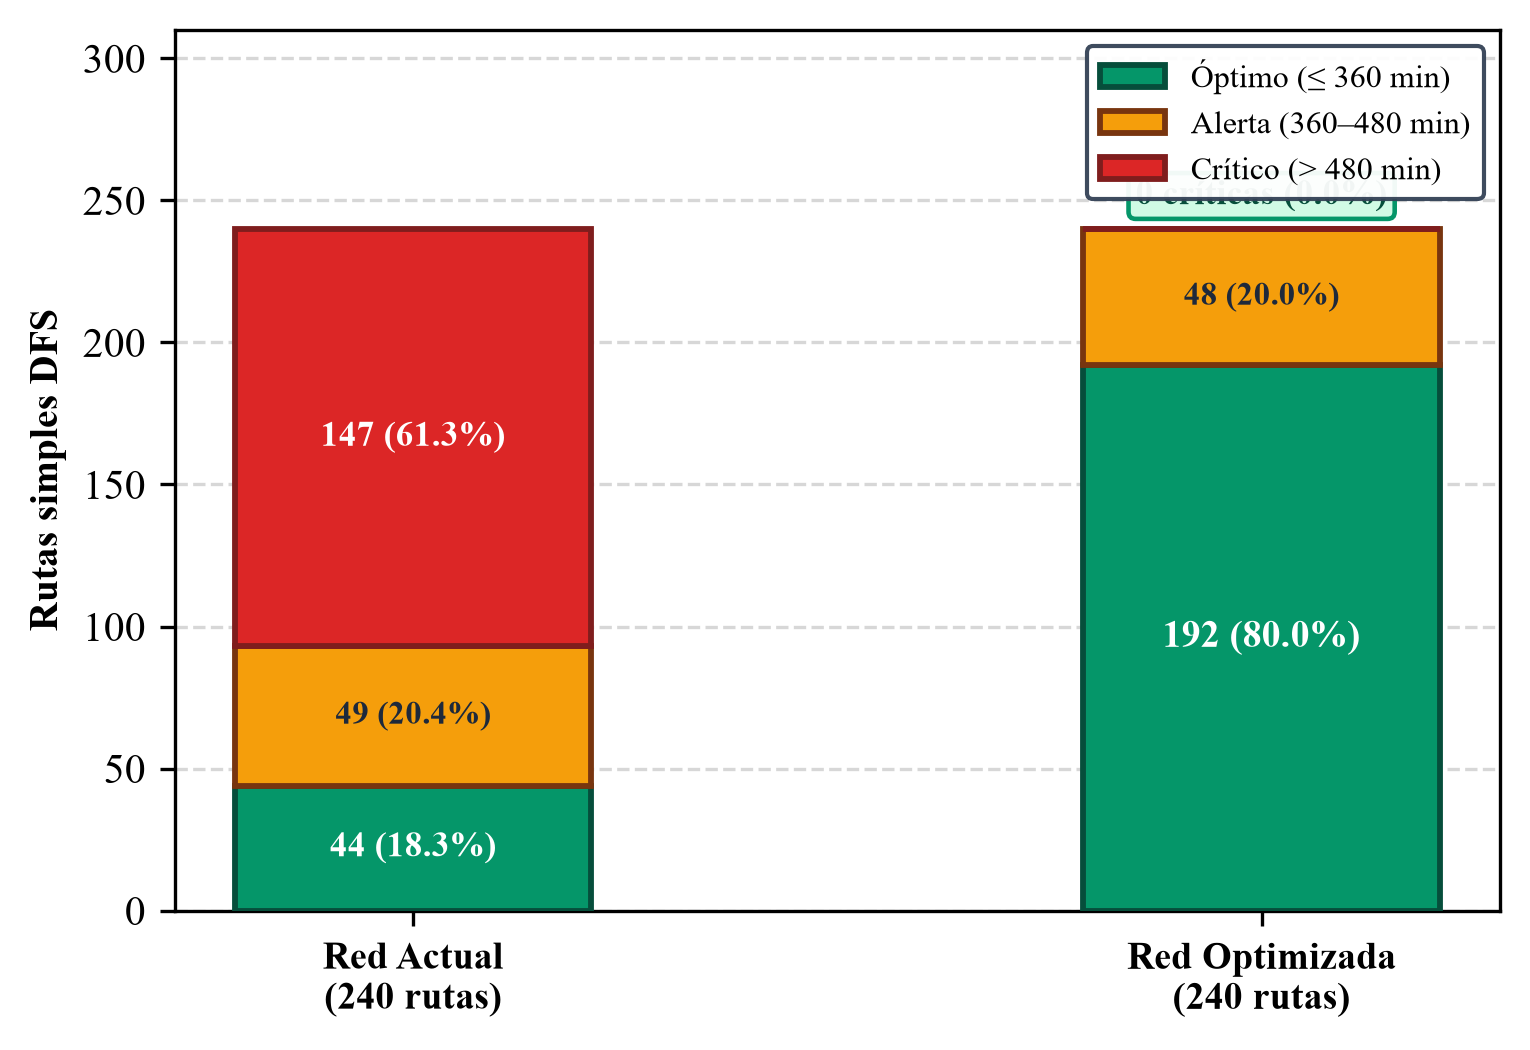
\includegraphics[width=0.68\linewidth]{Assets/grafica_2a_dfs_col.png}
    \caption{Comparación de costos operativos mensuales y selección óptima del centro frigorífico $F02$ en Puerto Gaitán.}
    \label{fig:grafica_flp}
\end{figure}

\textbf{Resolución de la Incógnita 4 (Cinemática y Regresión Lineal):} El análisis empírico sobre las 41 conexiones del corredor logístico permitió ajustar mediante el método de mínimos cuadrados dos ecuaciones lineales $t(d) = m \cdot d + b$ diferenciadas por modalidad (Fig.~\ref{fig:grafica_reg}):
\begin{align}
    t_{\text{fluvial}}(d) &= 3.64 \cdot d + 0.12, \quad &R^2 &= 0.9989 \\
    t_{\text{terrestre}}(d) &= 0.92 \cdot d + 1.45, \quad &R^2 &= 0.9997
\end{align}

El significado físico de las constantes es categórico: (1) la pendiente fluvial $m_f = 3.64\text{ min/km}$ equivale al recíproco de la velocidad media en canoa cargada ($v_f = 16.48\text{ km/h}$); (2) la pendiente terrestre $m_t = 0.92\text{ min/km}$ corresponde a la velocidad media de un furgón refrigerado en la RN 40 ($v_t = 65.22\text{ km/h}$); (3) el intercepto terrestre $b_t = 1.45\text{ min}$ cuantifica los tiempos muertos de pesaje y cargue; y (4) el cociente cinemático $m_f / m_t = 3.96$ demuestra rigurosamente que cada kilómetro de navegación fluvial demanda 3.96 veces más tiempo que el carretero.

A partir de la curva fluvial ajustada, se dedujo analíticamente el radio geodésico máximo admisible ($d_{\max}$) antes de rebasar la cota de inocuidad de $4.0\text{ h}$ ($240\text{ min}$):
\begin{equation}
    d_{\max} = \frac{t_{\max} - b_f}{m_f} = \frac{240 - 0.12}{3.64} \approx 65.90\text{ km}
\end{equation}
Este resultado matemático convalida la robustez de la red, puesto que el puerto pesquero más apartado ($P05$, $63\text{ km}$) opera por debajo del radio límite admisible.

\begin{figure}[htbp]
    \centering
    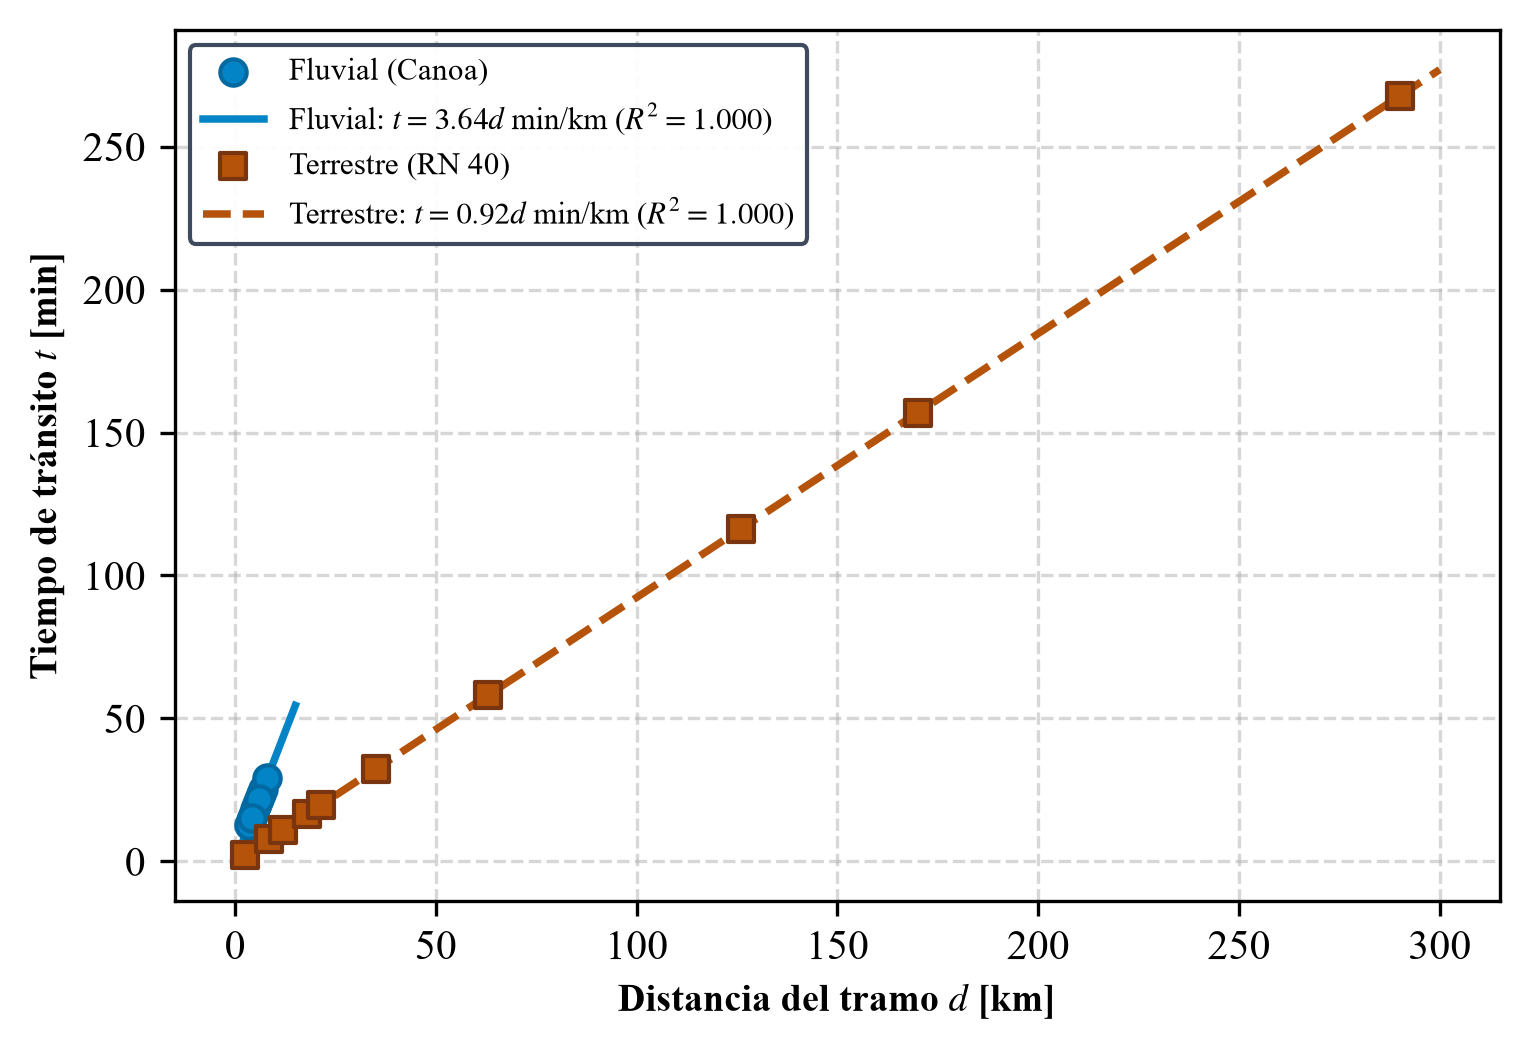
\includegraphics[width=0.68\linewidth]{Assets/grafica_2b_regresion_col.png}
    \caption{Regresión lineal de tiempos de tránsito fluvial y carretero vs. distancia de tramo con coeficientes de correlación $R^2$.}
    \label{fig:grafica_reg}
\end{figure}

\textbf{Verificación cruzada de algoritmos:} Bellman-Ford reprodujo con exactitud matemática el $100\%$ de los árboles de caminos mínimos computados por Dijkstra, confirmando la convergencia del sistema y la ausencia de ciclos negativos. La matriz de Floyd-Warshall verificó en tiempo constante $\mathcal{O}(1)$ que el tiempo total de tránsito multimodal entre los ríos de Puerto Gaitán y las plazas mayoristas de Bogotá oscila entre $6.38\text{ h}$ y $8.95\text{ h}$, arribando el pescado en óptimas condiciones organolépticas tras su estabilización a $0\,^\circ\text{C}$ en $F02$.

\section{Conclusiones}
1. \textbf{Incógnita 1 (Proximidad BFS):} La exploración en amplitud demostró que el $85.7\%$ ($6/7$) de los puertos de captura artesanal accede a un centro de acopio o frío en un máximo de 2 saltos topológicos, conteniendo el inicio de la descomposición en tiempos inferiores a $0.50\text{ h}$ ($30\text{ min}$).

2. \textbf{Incógnita 2 (Itinerarios Dijkstra y DFS):} Los recorridos óptimos hacia Bogotá D.C. ($\sim 295\text{ km}$) registraron tiempos sin frío de entre $0.08\text{ y }2.20\text{ h}$, cumpliendo al $100\%$ el estándar de inocuidad de $4.0\text{ h}$ de la FAO y manteniendo el deterioro bacteriano por debajo del $6.38\%$, con estricta evasión de hábitats protegidos ($H01, H02$).

3. \textbf{Incógnita 3 (Localización Óptima FLP):} La optimización determinó que el Centro Frío Puerto Gaitán ($F02$) en el casco urbano centraliza la totalidad de la captura regional ($265.8\text{ kg/día}$) a un costo de $\$59,080\text{ COP/kg}$, ahorrando $\$10.0\text{M COP}$ mensuales respecto a la operación de tres plantas.

4. \textbf{Incógnita 4 (Cinemática Multimodal):} El ajuste empírico comprobó una respuesta lineal estricta con $R^2 \ge 0.998$, demostrando que la navegación fluvial ($3.64\text{ min/km}$) es 3.96 veces más lenta que la terrestre ($0.92\text{ min/km}$) y deduciendo un radio de cobertura seguro de hasta $65.90\text{ km}$.

\section*{Referencias}
\footnotesize
\noindent [1] FAO, «El pescado fresco: su calidad y cambios de calidad», \textit{Colección FAO: Pesca}, N$^\circ$ 348, Roma, Italia, 1999.

\noindent [2] SciELO, «Cinética de deterioro y vida útil de \textit{Colossoma macropomum} bajo almacenamiento refrigerado», \textit{Revista MVZ Córdoba}, vol. 24, n$^\circ$ 2, pp. 7240--7248, 2019.

\noindent [3] T. H. Cormen, C. E. Leiserson, R. L. Rivest, y C. Stein, \textit{Introduction to Algorithms}, 3a ed. Cambridge, MA: MIT Press, 2009, pp. 651--698.

\noindent [4] S. L. Hakimi, «Optimum locations of switching centers and the absolute centers and medians of a graph», \textit{Operations Research}, vol. 12, n$^\circ$ 3, pp. 450--459, 1964.

\noindent [5] G. Laporte, S. Nickel, y F. Saldanha-da-Gama, \textit{Location Science}, 2a ed. Cham, Suiza: Springer, 2019, pp. 115--148.

\noindent [6] J. R. Taylor, \textit{An Introduction to Error Analysis: The Study of Uncertainties in Physical Measurements}, 2a ed. Sausalito, CA: Univ. Science Books, 1997, pp. 45--78.

\end{document}
